\section{UNIX e Linux}
\subsection{Storia}
Nel 1969 l' azienda di telecomunicazioni AT\&T sviluppa un ambiente di calcolo multiprogrammato e portabile per macchine di medie dimensioni, nel 1970 esce la prima versione di UNIX, un sistema operativo multiprogrammato e monoutente interamente sviluppato in assembly per il calcolatore PDP-7.
Lungo tutti gli anni '70 escono nuove versioni di UNIX con nuove caratteristiche e funzionalità tra le quali l' introduzione al supporto multiutente.

Nel 1973 esce una versione di UNIX interamente scritta in C, questo permette una elevata compatibilità in quanto potrebbe venire eseguito su qualsiasi architettura che metta a disposizione un compilatore, con le minime modifiche possibili.
Si diffonde pertanto nella comunità scientifica ed accademica principalmente per eseguire calcoli matematici e fisici.

Negli anni '80 iniziano a venire fuori varie versioni di UNIX, in particolare due famiglie:
\begin{itemize}
    \item Unix System V (dagli AT\&T laboratories)
    \item Unix Berkeley Software Distributions - BSD (dall' Università della California a Berkeley)
\end{itemize}
Nel 1988 in particolare la IEEE emette lo standard POSIX (Portable Operating Systems Interface) che definisce le caratteristiche relative alle modalità di utilizzo del sistema operativo.
Negli anni 90 anche UNIX e le sue versioni si uniformano a POSIX.

Nel 1991 inizia lo svilupo del kernel Linux che poi verrà integrato con le utility del progetto GNU (GNU's not UNIX) formando il sistema operativo GNU/Linux.
Il progetto GNU si deve a Richard Stallman mentre il kernel Linux si deve a Linus Torvalds, sono tutte componenti open source liberamente scaricabili dalla rete sotto licenza GPL.
Le principali caratteristiche di questi sistemi operativi sono la gestione multi-utente, il multithreading, la multiprogrammazione, inoltre abbiamo anche una forte estendibilità ed affidabilità date le estese community.

\subsection{Caratteristiche di UNIX/Linux}
\begin{figure}[H]
    \centering
    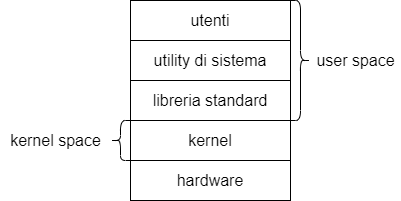
\includegraphics[width=200px]{images/13_UNIX_Linux/UNIX_stack.png}
\end{figure}
\begin{itemize}
    \item il kernel si occupa della gestione dei processi, della memoria, crea l' astrazione del file system e gestisce l' I/O
    \item la libreria standard fornisce dei wrapper programmer-friendly per system call del kernel
    \item le utility di sistema come shell, editor e compilatori forniscono all' utente gli utensili necessari per l' utilizzo del sistema operativo a pieno e per lo sviluppo dello stesso 
\end{itemize}

\subsubsection{Gestione dei processi}
Essendo un sistema operativo multiprogrammato UNIX deve gestire in qualche modo i suoi processi: sfrutta una politica a divisione di tempo.

Ogni processo in UNIX è un processo pesante con codice \emph{rientrante} cioè ha la sezione dati non condivisa mentre il codice condivisibile con altri processi dello stesso programma.
Fornisce un funzionamento dual mode in cui abbiamo processi utente (modalità user) e processi di sistema (modalità kernel).
Queste divisioni ci permettono di avere una diversa visibilità della memoria.

Per organizzare la condivisione del codice il sistema operativo ha una struttura dati detta \emph{text table} che contiene i puntatori alle sezioni di codice ed il numero di processi attualmente interessati alla porzione di codice, ogni record è detto \emph{text structure}.

Ovviamente anche in UNIX un processo è modellato in un Process Control Block (descrittore di processo), diviso in due strutture dati:
\begin{itemize}
    \item Process Structure: contiene le informazioni necessarie al sistema per la gestione del processo, deve pertanto rimanere sempre in memoria.
    Alcune informazioni contenute sono:
    \begin{itemize}
        \item PID
        \item stato del processo
        \item puntatore a dati e stack
        \item riferimento alla text structure
        \item informazioni utili allo scheduling come priorità, tempo di CPU, ed altro
        \item informazioni relative ai segnali come segnali inviati, ricevuti, handler custom, ecc
        \item puntatore al processo seguente nella coda
        \item puntatore alla user structure
    \end{itemize}
    \item User Structure: contiene le informazioni necessarie solo se il processo è residente in memoria centrale, può pertanto essere soggetto a swap.
    Alcune informazioni contenute sono:
    \begin{itemize}
        \item contesto del processo
        \item informazioni sulle risorse allocate dal processo come file aperti, ecc
        \item informazioni sulla gestione dei segnali
        \item ambiente del processo: directory di esecuzione, utente, gruppo, parametri passati al programma, path, ecc
    \end{itemize}
\end{itemize}
Tutti i PCB sono contenuti nella \emph{process table} che è di dimensione fissa, questo per porre un limite ai processi attivi contemporaneamente.


\subsubsection{Gestione della memoria}
Ogni processo ha la sua memoria raggruppabile in:
\begin{itemize}
    \item parte kernel
    \item parte utente
\end{itemize}
ma anche in:
\begin{itemize}
    \item parte swappable
    \item parte residente e non swappable
\end{itemize}
Es: la process table e la text table sono parte kernel residente, non possiamo spostarla nella swap.
User structure e stack kernel sono memoria kernel che possiamo swappare se il processo è vittima dell' algoritmo di swap.
Dati, codice e stack utente sono memoria utente e swappabile.


\subsubsection{Terminazione dei processi}
Un processo può terminare in maniera volontaria chiamando la system call exit, oppure in maniera involontaria a causa di interruzioni, segnali, tentativi di azioni illegali ed eccezioni.
Se il processo che termina aveva dei figli essi vengono adottati dal processo init, se il processo termina prima che il padre abbia chiamato la primitiva wait (per leggere lo stato di uscita del processo figlio) il processo va in stato zombie.


\subsubsection{Scheduling dei processi}
Ad ogni processo si assegna un valore di priorità in cui più il valore è piccolo e più alta è la priorità.
Proprio per questo meccanismo i processi utente hanno priorità $\geq 0$ mentre quelli sistema hanno tutti priorità $ < 0$.
Inoltre i processi sistema non possono essere interrotti in quanto girano con le interruzioni disabilitate per garantire l' atomicità.

Ogni livello di priorità ha una coda gestita con round robin, inoltre le priorità sono dinamiche e la priorità decresce all' aumentare del tempo di CPU utilizzato.


\subsubsection{Gestione della memoria}
Da BSD 3 in poi si ha la segmentazione paginata con paginazione a domanda.
Per gestire la memoria si usa una struttura dati detta \emph{Core map} che descrive lo stato di allocazione dei frame ed è usata durante i page-fault.
Si utilizza l' algoritmo second chance per cercare pagine da sostituire.

La sostituzione delle pagine è gestita da diversi processi di sistema secondo 3 parametri:
\begin{itemize}
    \item lotsfree: numero minimo di frame liberi per evitare paginazione
    \item minfree: numero minimo di frame liberi necessari per evitare lo swapping dei processi
    \item desfree: numero minimo di frame desiderabili
\end{itemize}
Il processo \emph{page-daemon} mantiene lotsfree pagine libere, è eseguito periodicamente per appunto tenere un tot di pagine libere, usa second chance.
Se non ci sono almeno minfree pagine parte il processo \emph{swapper} che libera tanti frame quanti ne servono per avere minfree pagine libere, esegue di fatto lo swap-out di un processo scelto, che non è quello che ha eseguito il page-fault.

Se chiamo swapper solo sulla condizione del valore di minfree rischio il trashing, per evitare ciò periodicamente calcolo la media dei frame liberi e se il numero di frame liberi scende sotto minfree ed il numero medio di frame liberi è minore di desfree faccio partire swapper.
Questo approccio mi permette di non avere delle chiamate nette quando si scende sotto minfree, così la curva dell' utilizzo delle pagine è più continua.

\subsection{File system}
\subsubsection{Organizzazione logica}
Abbiamo una organizzazione ad albero con la directory root che prende il nome /.
In UNIX ogni risorsa è un file, essi vengono caratterizzati in:
\begin{itemize}
    \item file ordinari
    \item directory
    \item dispositivi che sono file speciali e si trovano in directory particolari come \verb{/dev{ o \verb{/proc{
\end{itemize}

Ad ogni file è associato un nome ma può avere altri nomi simbolici (link), tuttavia ad ogni file è associato uno ed un solo descrittore di file, chiamato i-node, contenuto nella i-list, univocamente identificato da un i-number.

\subsubsection{Organizzazione fisica}
E' utilizzata una allocazione ad indice a più livelli, in realtà è ibrida per i file di piccole dimensioni.
Gestisce blocchi fisici da 512 a 4096 byte.

Il disco fisico è partizionato in 4 porzioni:
\begin{itemize}
    \item Boot Block: vi è posizionato il codice da caricare in memoria ed eseguire al boot del sistema
    \item SuperBlock: contiene le informazioni sui limiti delle 4 regioni, il puntatore a una lista dei blocchi liberi ed il puntatore ad una lista degli i-node liberi
    \item I-List: contiene la lista di tutti gli i-node, delle directory e dei file
    \item Data Blocks: è l' area del disco effettivamente disponibile per la memorizzazione dei file
\end{itemize}

\subsubsection{i-node}
E' il descrittore del file, tra gli attributi che ospita ci sono:
\begin{itemize}
    \item tipo di file: se ordinario, directory o file speciale
    \item proprietario, gruppo
    \item dimensione
    \item data
    \item 12 bit di protezione: read-write-execute per utente, gruppo ed altri
    \item numero di links: numero di pathname diverse che portano a questo file
    \item vettore di indirizzamento: 13 - 15 indirizzi di blocchi usati per l' accesso ai dati
\end{itemize}

\subsubsection{Indirizzamento}
Supponiamo di avere dei blocchi di dimensione 512 byte indirizzati su 32 bit, possiamo dire che 1 blocco contiene 128 indirizzi.

Nel descrittore di file abbiamo quindi 10 blocchi di dati che sono accessibili direttamente in quanto i primi 10 indirizzi nel vettore di indirizzamento puntano direttamente a dei blocchi.

L' undicesimo indirizzo del vettore è l' indice di un blocco indice, quindi tramite questo blocco possiamo indirizzarne altri 128.
Con questo metodo possiamo allocare file fino a 64 KByte (128 * 512 = 65536 byte) al costo di un solo blocco in più.

Il dodicesimo indirizzo del vettore contiene l' indice di un blocco indice di primo livello, questo significa che ogni blocco puntato da questo indice è a sua volta un blocco indice.
Possiamo quindi indirizzare 128*128 blocchi cioè file da 8Mbyte.
Questa è chiamata indirezione doppia e prevede due letture dal disco per leggere le due tabelle di indirezione da attraversare.

Il tredicesimo indirizzo del vettore contiene l' indice di blocchi con indirezione tripla, possiamo quindi indirizzare fino a 128*128*128 blocchi cioè 1GB.
In questa politica dobbiamo eseguire 3 letture su disco per leggere i 3 blocchi indice da navigare.

Su sistemi con 13 elementi nel vettore di indirizzamento possiamo allocare file fino a 1GB+8MB+64KB+5KB.

Se portiamo il vettore a 14 elementi arriviamo a file di oltre 128GB e con 15 ancora di più.


\subsubsection{Directory}
Una directory contiene file ed altre directory quindi il suo descrittore è una tabella che associa i nomi simbolici del contenuto e l' indice dell' i-node nella i-list.

\subsubsection{Accesso a file}
UNIX permette l' accesso sequenziale attraverso un \emph{I/O pointer} che indica la posizione corrente nella lettura/scrittura del file.
Non abbiamo una strutturazione particolare, un file è un flusso di byte.

Permette svariati modi di accesso: lettura, scrittura, lettura e scrittura, append ed altri ma l' accesso è subordinato all' operazione di apertura.


\subsubsection{Strutture dati del kernel per l' accesso ai file}
Ogni processo nel proprio descrittore ha una tabella dei file aperti, ogni elemento rappresenta un file aperto dal processo individuato da un indice intero detto \emph{file descriptor}.

NB: i file descriptor 0, 1 e 2 rappresentano rispettivamente lo standard input, lo standard output e lo standard error e sono aperti automaticamente all' avvio del processo.

La User Area del processo contiene i file descriptor che hanno i puntatori alla tabella dei file aperti di sistema dove per ogni file aperto c'è un descrittore con due campi:
\begin{itemize}
    \item IO-pointer del file: indice da usare per l' accesso fisico al disco
    \item puntatore all' i-node nella tabella dei file attivi
\end{itemize}

\begin{figure}[H]
    \centering
    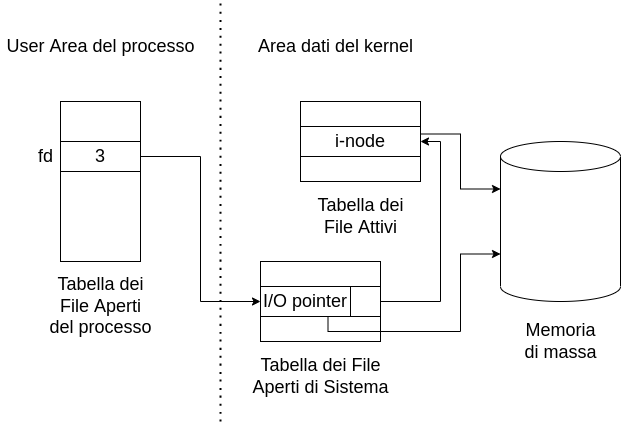
\includegraphics[width=330px]{images/13_UNIX_Linux/kernel_file_data_structure.png}
\end{figure}

Si noti che se apro lo stesso file più volte avrò IO-pointer diversi ma l' i-node è singolo nella tabella dei file attvi.

\subsubsection{Apertura di un file: open()}
Quando l' utente chiede di aprire un file devo quindi:
\begin{itemize}
    \item copiare l' i-node del file dalla memoria di massa alla tabela dei file attivi, se non c'è già
    \item aggiungere una entry nella tabella dei file aperti di sistema con il puntatore all'i-node ed un IO-pointer azzerato
    \item aggiungere una entry nella tabella dei file aperti del processo ed assegnare un file descriptor a questa entry
    \item ritornare l' intero file descriptor all' utente in modo che possa usarlo
\end{itemize}
Quando apriamo un file oltre ad aprirlo genericamente lo apriamo in una determinata modalità, quindi nella open bisogna controllare che l' utente possa effettivamente usare quel file nella modalità che sta richiedendo.

\subsubsection{System call per l' accesso ai file}
\begin{itemize}
    \item \verb{open(){: serve per allocare le strutture dati relative ai file all' interno del sistema operativo.
    Ovviamente prima di eseguire l' apertura effettiva vanno controllati i permessi dell' utente relativi al file con il quale interagire.
    
    \item \verb{close(){: permette di chiudere un file fornendogli il file descriptor associato.
    Se la chiamata ha successo il file viene memorizzato sul disco e vengono eliminati gli elementi associati ad esso nelle tabelle del kernel.
    
    \item \verb{read{ e \verb{write{: ogni operazione di lettura o scrittura agisce sul file in maniera sequenziale a partire dalla posizione corrente dettata da I/O pointer.
    Le operazioni sono atomiche e sono sincrone cioè il processo viene stoppato in attesa del completamento dell' operazione.
    Possiamo alternare letture e scritture se il file è stato aperto in modalità congruente.
\end{itemize}


